% ============================================================================
% EMSI AGENTIC PRESENTATION TEMPLATE
% ----------------------------------------------------------------------------
% PURPOSE
%   This file is a reusable visual model for school projects, internships,
%   final-year projects, research presentations and technical demonstrations.
%
% AI CONTRACT
%   - Preserve the design system, EMSI identity, layout helpers and TikZ styles.
%   - Replace all placeholder content with project facts from the supplied YAML.
%   - Remove irrelevant modules rather than leaving empty slides.
%   - Keep partner/company branding conditional.
%   - Prefer diagrams where they explain better than text.
% ============================================================================

\documentclass[aspectratio=169]{beamer}

% ----------------------------------------------------------------------------
% 1. COMPATIBLE ENGINE AND PACKAGES -- normally preserve
% ----------------------------------------------------------------------------
\usepackage{iftex}
\ifPDFTeX
  \usepackage[utf8]{inputenc}
  \usepackage[T1]{fontenc}
  \usepackage{lmodern}
\else
  \usepackage{fontspec}
  \defaultfontfeatures{Ligatures=TeX}
  \setsansfont{Latin Modern Sans}
\fi

\usepackage{textpos}
\usepackage{graphicx}
\graphicspath{{./}{assets/}{assets/logos/}{assets/images/}{assets/user/}}
\usepackage{wrapfig}
\usepackage{tikz}
\usetikzlibrary{arrows.meta,backgrounds,calc,fit,matrix,positioning,shapes.geometric,shapes.symbols}
\usepackage{amsmath,amssymb}
\usepackage[framemethod=TikZ]{mdframed}
\usepackage{caption}
\usepackage{array}
\usepackage{pgfgantt}
\usepackage{pgf-umlsd}
\usepackage{listings}
\usepackage{adjustbox}
\usepackage{xparse}
\hfuzz=3pt

\usetheme{Boadilla}
\usecolortheme{default}
\setbeamercolor{structure}{fg=blue!65!black}
\setbeamercolor{alerted text}{fg=red!75!black}
\setbeamercolor{block title}{bg=blue!12,fg=black}
\setbeamercolor{block body}{bg=blue!3,fg=black}
\setbeamertemplate{caption}[numbered]
\setbeamertemplate{navigation symbols}{}

% ----------------------------------------------------------------------------
% 2. PERMANENT VISUAL SYSTEM -- preserve and reuse
% ----------------------------------------------------------------------------
\tikzset{
  actor/.style={draw, ellipse, minimum height=1.5em, minimum width=3em, align=center},
  usecase/.style={draw, ellipse, minimum height=2.5em, minimum width=3.2cm, align=center},
  stage/.style={draw, thick, rounded corners=4pt, minimum width=2.5cm,
                minimum height=1.25cm, inner sep=5pt, align=center, font=\small\bfseries},
  component/.style={draw, rounded corners=3pt, minimum width=2.15cm,
                    minimum height=0.9cm, align=center, font=\scriptsize},
  datastore/.style={draw, cylinder, shape border rotate=90, aspect=0.28,
                    minimum width=1.9cm, minimum height=1.05cm, align=center, font=\scriptsize},
  boundary/.style={draw, dashed, rounded corners=5pt, inner sep=9pt},
  flow/.style={-{Latex[length=2.5mm]}, thick, draw=gray!75!black},
  criticalflow/.style={-{Latex[length=2.8mm]}, very thick, draw=red!75!black},
  note/.style={font=\tiny, text=gray!80!black, align=center},
  decision/.style={draw, diamond, aspect=2.2, align=center, font=\scriptsize},
  result/.style={draw, rounded corners=5pt, fill=green!12, minimum width=2.3cm,
                 minimum height=1cm, align=center, font=\scriptsize\bfseries}
}

% PERT node: ID/style/position/title/earliest/latest
\newcommand{\pertnode}[6]{%
  \node[draw, thick, minimum width=2cm, minimum height=1.15cm,
        fill=white, inner sep=0pt, outer sep=2pt, #2] (#1) at #3 {};%
  \node[font=\scriptsize\bfseries, anchor=center]
        at ([yshift=0.18cm]#1.center) {#4};%
  \draw[thick] ([yshift=-0.08cm]#1.west) -- ([yshift=-0.08cm]#1.east);%
  \draw[thick] ([yshift=-0.08cm]#1.center) -- (#1.south);%
  \node[font=\tiny, anchor=center]
        at ([xshift=-0.5cm, yshift=-0.36cm]#1.center) {#5};%
  \node[font=\tiny, anchor=center]
        at ([xshift=0.5cm, yshift=-0.36cm]#1.center) {#6};%
}

% Small explanation strip retained from the reference presentation.
\newcommand{\slidepurpose}[2]{%
  \vspace*{-0.23cm}
  \begin{center}
  {\tiny
  \setlength{\fboxsep}{3pt}%
  \setlength{\fboxrule}{0.6pt}%
  \fcolorbox{black!55}{gray!10}{%
  \parbox{\dimexpr0.97\linewidth-2\fboxsep-2\fboxrule\relax}{\raggedright
  \textbf{Role:} #1 \hfill \textbf{Project Stage:} #2}}}
  \end{center}
  \vspace{0.03cm}
}

\newcommand{\defitem}[2]{\textbf{#1}: #2\par\vspace{0.32em}}

% Safe image placeholder: the deck still compiles when an optional asset is absent.
\newcommand{\placeholdergraphic}[2][0.62\textheight]{%
  \fbox{\begin{minipage}[c][#1][c]{0.88\linewidth}
  \centering\small\textbf{Asset placeholder}\\[0.25cm]
  \texttt{#2}
  \end{minipage}}
}

% Figure helper with graceful fallback.
\newcommand{\solutionfigure}[2]{%
  \begin{center}
  \begin{minipage}[c][0.67\textheight][c]{\linewidth}
  \centering
  \IfFileExists{#1}{%
    \includegraphics[width=0.98\linewidth,height=0.61\textheight,keepaspectratio]{#1}%
  }{\placeholdergraphic[0.51\textheight]{#1}}
  \end{minipage}
  \vspace{0.06cm}
  {\captionsetup{type=figure,font=tiny,justification=centering}
  \captionof{figure}{#2}%
  \addcontentsline{lof}{figure}{\protect\numberline{\thefigure}{#2}}%
  \recordfigureentry{#2}}
  \end{center}
}

% TikZ figure helper retained from the reference presentation.
\newcommand{\tikzsolutionfigure}[2]{%
  \begin{center}
  \begin{minipage}[c][0.64\textheight][c]{\linewidth}
  \centering
  \begin{adjustbox}{max width=0.96\linewidth, max height=0.62\textheight}
  #1
  \end{adjustbox}
  \end{minipage}
  \vspace{0.06cm}
  {\captionsetup{type=figure,font=tiny,justification=centering}
  \captionof{figure}{#2}%
  \addcontentsline{lof}{figure}{\protect\numberline{\thefigure}{#2}}%
  \recordfigureentry{#2}}
  \end{center}
}

% Dynamic figure list retained from the reference presentation.
\renewcommand{\listfigurename}{List of Figures}
\makeatletter
\@ifundefined{tf@lof}{\newwrite\tf@lof}{}
\immediate\openout\tf@lof=\jobname.lof\relax
\newcommand{\storedfigurelist}{}
\newcommand{\figurelistentry}[3]{%
  \g@addto@macro\storedfigurelist{\noindent \textbf{Figure #1.} #2 \dotfill #3\par}%
}
\newcommand{\recordfigureentry}[1]{%
  \protected@write\@auxout{}{\string\figurelistentry{\thefigure}{#1}{\thepage}}%
}
\newcommand{\dynamiclistoffigures}{%
  \begingroup
  \parindent=0pt
  \parskip=0.35em
  \footnotesize
  \ifx\storedfigurelist\@empty
    \textit{No figures listed yet.}%
  \else
    \storedfigurelist
  \fi
  \endgroup
}
\makeatother

% ----------------------------------------------------------------------------
% 3. PRESENTATION VARIABLES -- AI replaces these values
% ----------------------------------------------------------------------------
\newcommand{\PresentationTitle}{[PROJECT TITLE]}
\newcommand{\PresentationShortTitle}{Project Presentation}
\newcommand{\PresentationSubtitle}{[OPTIONAL SUBTITLE]}
\newcommand{\PresenterNames}{[PRESENTER NAME(S)]}
\newcommand{\AcademicSupervisor}{[ACADEMIC SUPERVISOR]}
\newcommand{\PresenterEmail}{[EMAIL]}
\newcommand{\Programme}{[PROGRAMME / LEVEL]}
\newcommand{\AcademicYear}{[ACADEMIC YEAR]}
\newcommand{\PresentationDate}{[DATE]}
\newcommand{\PresentationLocation}{[LOCATION]}
\newcommand{\InstitutionName}{EMSI}
\newcommand{\SchoolLogoPath}{assets/logos/emsi-logo.png}

% Partner/company branding is optional.
\newif\ifhaspartner
\haspartnerfalse
\newcommand{\PartnerName}{[PARTNER NAME]}
\newcommand{\PartnerDepartment}{[DEPARTMENT]}
\newcommand{\PartnerSupervisor}{[PARTNER SUPERVISOR]}
\newcommand{\PartnerLogoPath}{assets/logos/partner-logo.png}

% Change \haspartnerfalse to \haspartnertrue only when organisation.enabled=true.

\title[\PresentationShortTitle]{\PresentationTitle}
\subtitle{\PresentationSubtitle}
\author[\PresenterNames]{\PresenterNames\inst{1}}
\institute[EMSI]{%
  \inst{1}\InstitutionName, \Programme\\
  \ifhaspartner
    \textbf{Organisation:} \PartnerName{} -- \PartnerDepartment\\
    \textbf{Organisation Supervisor:} \PartnerSupervisor\\
  \fi
  \textbf{Academic Supervisor:} \AcademicSupervisor\\
  \PresenterEmail
}
\date[\AcademicYear]{\PresentationLocation, \PresentationDate}

% EMSI remains in a fixed position. The partner logo is conditional.
\titlegraphic{%
  \begin{tikzpicture}[remember picture,overlay]
    \node[anchor=north east,xshift=-0.45cm,yshift=-0.35cm] at (current page.north east) {%
      \IfFileExists{\SchoolLogoPath}{%
        \includegraphics[height=0.72cm]{\SchoolLogoPath}%
      }{%
        \fbox{\scriptsize\bfseries EMSI}%
      }%
    };
    \ifhaspartner
      \node[anchor=north west,xshift=0.45cm,yshift=-0.35cm] at (current page.north west) {%
        \IfFileExists{\PartnerLogoPath}{%
          \includegraphics[height=0.95cm,width=2.6cm,keepaspectratio]{\PartnerLogoPath}%
        }{%
          \fbox{\scriptsize Partner Logo}%
        }%
      };
    \fi
  \end{tikzpicture}%
}

\AtBeginSection[]{%
  \begin{frame}
    \frametitle{Table of Contents}
    \small
    \tableofcontents[currentsection]
  \end{frame}
}

% ----------------------------------------------------------------------------
% 4. SLIDE MODULE CATALOGUE
% ----------------------------------------------------------------------------
% AI MODULE RULES
%   Keep only the slides that support the supplied project and duration.
%   Reorder modules to fit the selected presentation archetype.
%   Replace all [PLACEHOLDER] text. Never leave explanatory AI comments in the
%   audience-facing deck.
% ----------------------------------------------------------------------------

\begin{document}

% MODULE: title -- always include
\begin{frame}
  \titlepage
\end{frame}

% MODULE: navigation -- normally include for 10+ slides
\begin{frame}{Table of Contents}
  \slidepurpose{Present the selected narrative and section order}{Navigation / global framing}
  \small
  \tableofcontents
\end{frame}

% MODULE: list of figures -- include only when several meaningful figures exist
\begin{frame}[allowframebreaks]{List of Figures}
  \slidepurpose{List the diagrams and figures used in the presentation}{Navigation / global framing}
  \dynamiclistoffigures
\end{frame}

\section{Project Framing}

% MODULE: organisation overview -- delete when organisation.enabled=false
\ifhaspartner
\begin{frame}{Organisation and Project Context}
  \slidepurpose{Position the organisation, department and assigned context}{Context}
  \begin{columns}[c]
    \begin{column}{0.62\textwidth}
      \small
      \defitem{Organisation}{\PartnerName}
      \defitem{Department}{\PartnerDepartment}
      \defitem{Project context}{[WHY THIS WORK EXISTS INSIDE THE ORGANISATION]}
      \defitem{Assigned mission}{[CONCISE MISSION]}
    \end{column}
    \begin{column}{0.34\textwidth}
      \centering
      \IfFileExists{\PartnerLogoPath}{\includegraphics[width=0.8\linewidth]{\PartnerLogoPath}}{\placeholdergraphic[0.25\textheight]{\PartnerLogoPath}}
    \end{column}
  \end{columns}
\end{frame}
\fi

% MODULE: problem statement -- normally include
\begin{frame}{Problem Statement}
  \slidepurpose{State the concrete need and the central question}{Scientific framing}
  \begin{alertblock}{Central Question}
    [WRITE ONE PRECISE, PROJECT-SPECIFIC QUESTION.]
  \end{alertblock}
  \vspace{0.15cm}
  \small
  \defitem{Current limitation}{[WHAT DOES NOT WORK TODAY]}
  \defitem{Expected outcome}{[WHAT SUCCESS LOOKS LIKE]}
\end{frame}

% MODULE: problem segmentation -- excellent candidate for TikZ
\begin{frame}{Segmentation of the Problem}
  \slidepurpose{Break the problem into distinct solvable stages}{Scientific framing}
  \tikzsolutionfigure{
  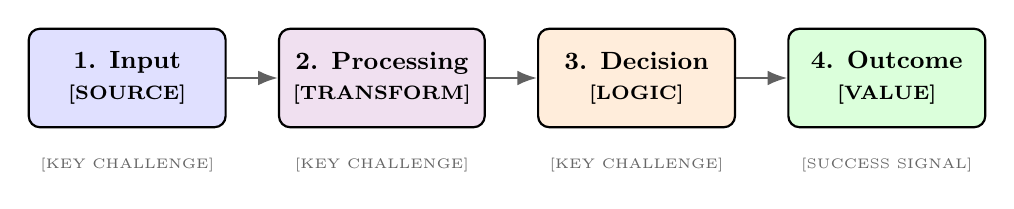
\begin{tikzpicture}[node distance=0.9cm and 0.65cm]
    \node[stage,fill=blue!12] (a) {1. Input\\{\scriptsize [SOURCE]}};
    \node[stage,fill=violet!12,right=of a] (b) {2. Processing\\{\scriptsize [TRANSFORM]}};
    \node[stage,fill=orange!14,right=of b] (c) {3. Decision\\{\scriptsize [LOGIC]}};
    \node[stage,fill=green!14,right=of c] (d) {4. Outcome\\{\scriptsize [VALUE]}};
    \draw[flow] (a)--(b);
    \draw[flow] (b)--(c);
    \draw[flow] (c)--(d);
    \node[note,below=0.25cm of a]{[KEY CHALLENGE]};
    \node[note,below=0.25cm of b]{[KEY CHALLENGE]};
    \node[note,below=0.25cm of c]{[KEY CHALLENGE]};
    \node[note,below=0.25cm of d]{[SUCCESS SIGNAL]};
  \end{tikzpicture}
  }{General problem decomposition. Replace with the real project stages.}
\end{frame}

\section{Methodology and Planning}

% MODULE: methodology -- include only when relevant
\begin{frame}{Methodology}
  \slidepurpose{Show how the work was organised and iterated}{Organisation / planning}
  \centering
  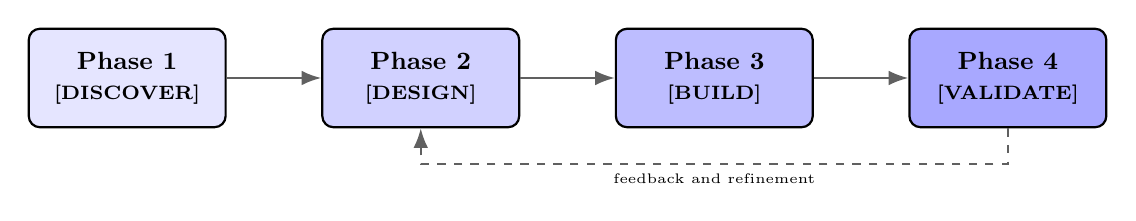
\begin{tikzpicture}[node distance=1.2cm]
    \node[stage,fill=blue!10] (p1) {Phase 1\\{\scriptsize [DISCOVER]}};
    \node[stage,fill=blue!18,right=of p1] (p2) {Phase 2\\{\scriptsize [DESIGN]}};
    \node[stage,fill=blue!26,right=of p2] (p3) {Phase 3\\{\scriptsize [BUILD]}};
    \node[stage,fill=blue!34,right=of p3] (p4) {Phase 4\\{\scriptsize [VALIDATE]}};
    \draw[flow] (p1)--(p2);
    \draw[flow] (p2)--(p3);
    \draw[flow] (p3)--(p4);
    \draw[flow,dashed] (p4.south) -- ++(0,-0.45) -| (p2.south)
      node[pos=.25,below,font=\tiny]{feedback and refinement};
  \end{tikzpicture}
  \vspace{0.35cm}
  \small [EXPLAIN WHY THIS METHODOLOGY FITS THE PROJECT.]
\end{frame}

% MODULE: task table -- include when tasks are supplied
\begin{frame}{Project Management --- Task Table}
  \slidepurpose{Summarise work packages, duration and dependencies}{Organisation / planning}
  \scriptsize
  \renewcommand{\arraystretch}{1.18}
  \begin{adjustbox}{max width=0.98\textwidth}
  \begin{tabular}{|c|p{6.1cm}|c|p{4.2cm}|}
    \hline
    \textbf{ID} & \textbf{Task} & \textbf{Duration} & \textbf{Predecessor / relation} \\ \hline
    A & [TASK A] & [N] d & --- \\ \hline
    B & [TASK B] & [N] d & A (FS) \\ \hline
    C & [TASK C] & [N] d & A (FS) \\ \hline
    D & [TASK D] & [N] d & B, C (FS) \\ \hline
  \end{tabular}
  \end{adjustbox}
  \vspace{0.2cm}
  \tiny Replace this sample only with supplied tasks and dependencies.
\end{frame}

% MODULE: PERT -- remove unless requested and enough planning data exists
\begin{frame}{Project Management --- PERT Network}
  \slidepurpose{Visualise dependencies, dates and the critical path}{Organisation / planning}
  \tikzsolutionfigure{
  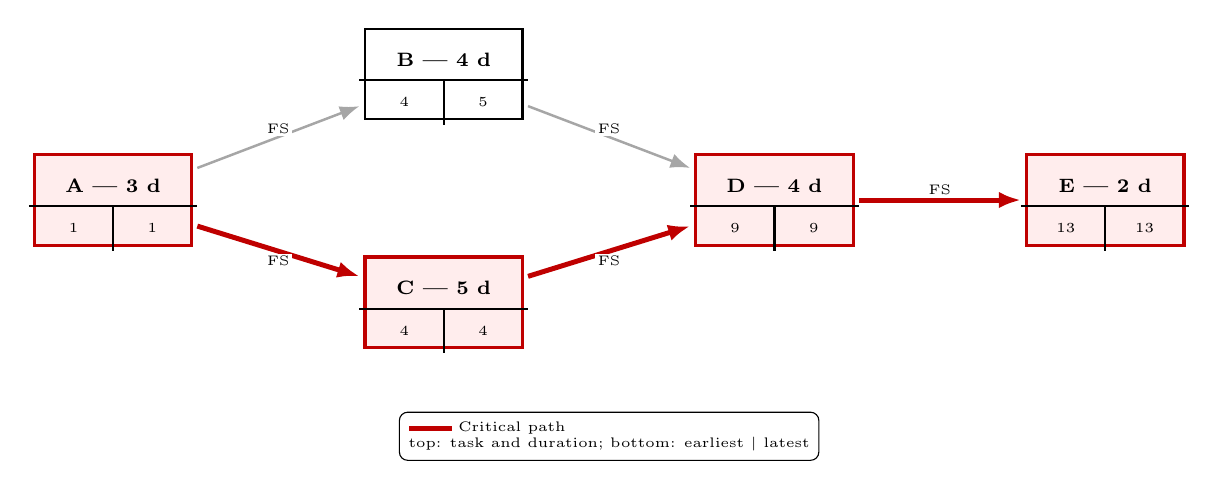
\begin{tikzpicture}[x=1.05cm,y=1cm,
    link/.style={-{Latex[length=2.5mm]},line width=.9pt,draw=gray!70},
    clink/.style={-{Latex[length=2.8mm]},line width=1.8pt,draw=red!75!black},
    rel/.style={font=\tiny,fill=white,inner sep=1pt}]
    \pertnode{A}{draw=red!75!black,very thick,fill=red!7}{(0,0)}{A --- 3 d}{1}{1}
    \pertnode{B}{}{(4,1.6)}{B --- 4 d}{4}{5}
    \pertnode{C}{draw=red!75!black,very thick,fill=red!7}{(4,-1.3)}{C --- 5 d}{4}{4}
    \pertnode{D}{draw=red!75!black,very thick,fill=red!7}{(8,0)}{D --- 4 d}{9}{9}
    \pertnode{E}{draw=red!75!black,very thick,fill=red!7}{(12,0)}{E --- 2 d}{13}{13}
    \draw[link] (A)--node[rel,above]{FS}(B);
    \draw[clink] (A)--node[rel,below]{FS}(C);
    \draw[link] (B)--node[rel,above]{FS}(D);
    \draw[clink] (C)--node[rel,below]{FS}(D);
    \draw[clink] (D)--node[rel,above]{FS}(E);
    \node[draw,rounded corners=3pt,fill=white,align=left,font=\tiny] at (6,-3.0) {
      \textcolor{red!75!black}{\rule{0.55cm}{2pt}} Critical path\\
      top: task and duration; bottom: earliest \textbar{} latest
    };
  \end{tikzpicture}
  }{Generic PERT pattern. Replace only with validated planning data.}
\end{frame}

% MODULE: Gantt -- remove unless requested and dates/durations exist
\begin{frame}{Project Management --- Gantt Chart}
  \slidepurpose{Project the validated tasks onto a readable timeline}{Organisation / planning}
  \centering
  \begin{adjustbox}{max width=0.98\textwidth,max totalheight=0.76\textheight}
  \begin{ganttchart}[
    hgrid,vgrid,x unit=.38cm,y unit chart=.55cm,y unit title=.5cm,
    title label font=\scriptsize\bfseries,bar label font=\scriptsize,
    bar/.append style={fill=blue!18,draw=blue!65!black},
    group/.append style={fill=black!10,draw=black!65},
    link/.style={-Latex,draw=black!60}]{1}{20}
    \gantttitle{Project Timeline}{20}\\
    \gantttitle{W1}{5}\gantttitle{W2}{5}\gantttitle{W3}{5}\gantttitle{W4}{5}\\
    \ganttgroup{Analysis}{1}{5}\\
    \ganttbar[name=a]{A Requirements}{1}{3}\\
    \ganttbar[name=b]{B Design}{4}{7}\\
    \ganttgroup{Delivery}{8}{20}\\
    \ganttbar[name=c]{C Implementation}{8}{15}\\
    \ganttbar[name=d]{D Validation}{16}{18}\\
    \ganttbar[name=e]{E Presentation}{19}{20}\\
    \ganttlink{a}{b}\ganttlink{b}{c}\ganttlink{c}{d}\ganttlink{d}{e}
  \end{ganttchart}
  \end{adjustbox}
\end{frame}

\section{Design and Implementation}

% MODULE: architecture -- use when a system or process has components
\begin{frame}{Proposed Architecture}
  \slidepurpose{Show boundaries, components, data flow and responsibilities}{Design}
  \tikzsolutionfigure{
  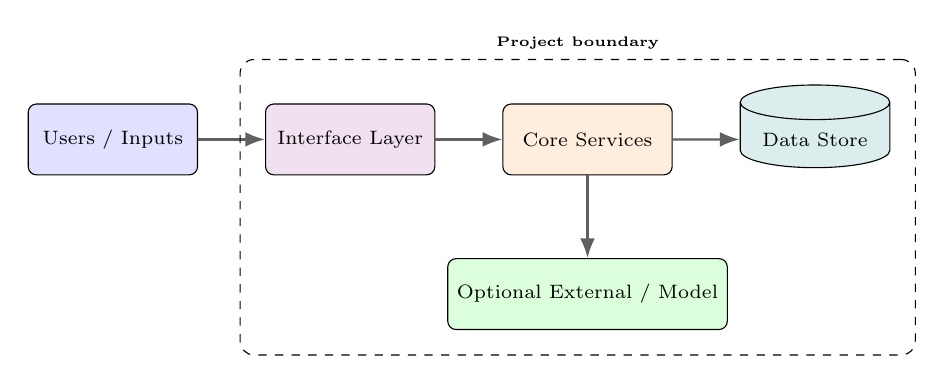
\begin{tikzpicture}[node distance=1.05cm and 0.85cm]
    \node[component,fill=blue!12] (client) {Users / Inputs};
    \node[component,fill=violet!12,right=of client] (interface) {Interface Layer};
    \node[component,fill=orange!13,right=of interface] (logic) {Core Services};
    \node[datastore,fill=teal!14,right=of logic] (data) {Data Store};
    \node[component,fill=green!14,below=of logic] (external) {Optional External / Model};
    \draw[flow] (client)--(interface);
    \draw[flow] (interface)--(logic);
    \draw[flow] (logic)--(data);
    \draw[flow] (logic)--(external);
    \node[boundary,fit=(interface)(logic)(data)(external),label={[font=\tiny\bfseries]above:Project boundary}] {};
  \end{tikzpicture}
  }{Reusable architecture grammar. Replace components with the real system.}
\end{frame}

% MODULE: workflow -- use for processing pipelines or user journeys
\begin{frame}{Core Workflow}
  \slidepurpose{Explain the most important end-to-end interaction}{Implementation}
  \centering
  \begin{adjustbox}{max width=0.94\linewidth}
  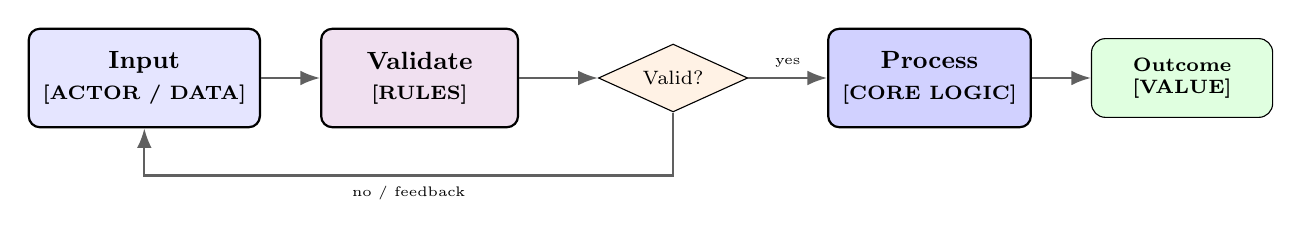
\begin{tikzpicture}[node distance=0.75cm]
    \node[stage,fill=blue!10] (w1) {Input\\{\scriptsize [ACTOR / DATA]}};
    \node[stage,fill=violet!12,right=of w1] (w2) {Validate\\{\scriptsize [RULES]}};
    \node[decision,fill=orange!10,right=1cm of w2] (w3) {Valid?};
    \node[stage,fill=blue!18,right=1cm of w3] (w4) {Process\\{\scriptsize [CORE LOGIC]}};
    \node[result,right=of w4] (w5) {Outcome\\{\scriptsize [VALUE]}};
    \draw[flow] (w1)--(w2);
    \draw[flow] (w2)--(w3);
    \draw[flow] (w3)--node[above,font=\tiny]{yes}(w4);
    \draw[flow] (w4)--(w5);
    \draw[flow] (w3.south)--++(0,-.8)-|node[pos=.25,below,font=\tiny]{no / feedback}(w1.south);
  \end{tikzpicture}
  \end{adjustbox}
\end{frame}

% MODULE: technology choices -- include only technologies actually used
\begin{frame}{Technology Choices}
  \slidepurpose{Connect each technology to a concrete responsibility}{Implementation}
  \centering
  \begin{adjustbox}{max width=0.9\linewidth}
  
\begin{tikzpicture}[node distance=.65cm]
    \node[component,fill=blue!12] (t1) {[TECH 1]\\\tiny interface};
    \node[component,fill=violet!12,right=of t1] (t2) {[TECH 2]\\\tiny application};
    \node[component,fill=orange!12,right=of t2] (t3) {[TECH 3]\\\tiny data};
    \node[component,fill=green!12,right=of t3] (t4) {[TECH 4]\\\tiny deployment};
    \draw[flow] (t1)--(t2);
    \draw[flow] (t2)--(t3);
    \draw[flow] (t3)--(t4);
  \end{tikzpicture}
  \end{adjustbox}
  \vspace{0.25cm}
  \small Each technology must map to a real project responsibility.
\end{frame}

% MODULE: implementation evidence -- use screenshots or code sparingly
\begin{frame}{Implementation Highlight}
  \slidepurpose{Demonstrate one important implemented capability}{Implementation}
  \solutionfigure{assets/images/implementation-highlight.png}{Replace with a real screenshot, interface, benchmark or implementation figure.}
\end{frame}

\section{Validation and Results}

% MODULE: testing
\begin{frame}{Validation Strategy}
  \slidepurpose{Show how correctness, quality and constraints were verified}{Validation}
  \centering
  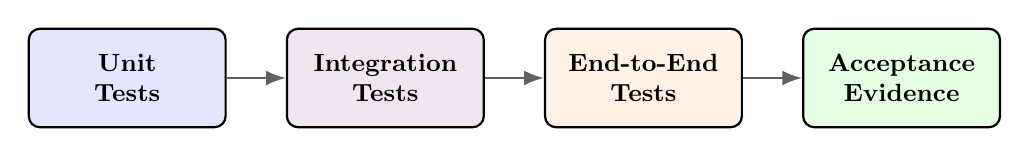
\begin{tikzpicture}[node distance=.75cm]
    \node[stage,fill=blue!10] (u) {Unit\\Tests};
    \node[stage,fill=violet!10,right=of u] (i) {Integration\\Tests};
    \node[stage,fill=orange!10,right=of i] (e) {End-to-End\\Tests};
    \node[stage,fill=green!10,right=of e] (a) {Acceptance\\Evidence};
    \draw[flow] (u)--(i);\draw[flow] (i)--(e);\draw[flow] (e)--(a);
  \end{tikzpicture}
  \vspace{0.35cm}
  \small [REPLACE WITH TESTS ACTUALLY PERFORMED AND THEIR EVIDENCE.]
\end{frame}

% MODULE: results -- omit or mark missing when no real results exist
\begin{frame}{Results}
  \slidepurpose{Present verified outcomes against the stated objectives}{Validation}
  \begin{columns}[T]
    \begin{column}{0.48\textwidth}
      \begin{block}{Delivered}
        \small
        \begin{itemize}
          \item \texttt{[RESULT 1]}
          \item \texttt{[RESULT 2]}
          \item \texttt{[RESULT 3]}
        \end{itemize}
      \end{block}
    \end{column}
    \begin{column}{0.48\textwidth}
      \begin{alertblock}{Limits}
        \small
        \begin{itemize}
          \item \texttt{[LIMITATION 1]}
          \item \texttt{[LIMITATION 2]}
        \end{itemize}
      \end{alertblock}
    \end{column}
  \end{columns}
\end{frame}

% MODULE: roadmap
\begin{frame}{Roadmap}
  \slidepurpose{Separate delivered scope from realistic future work}{Closure}
  \centering
  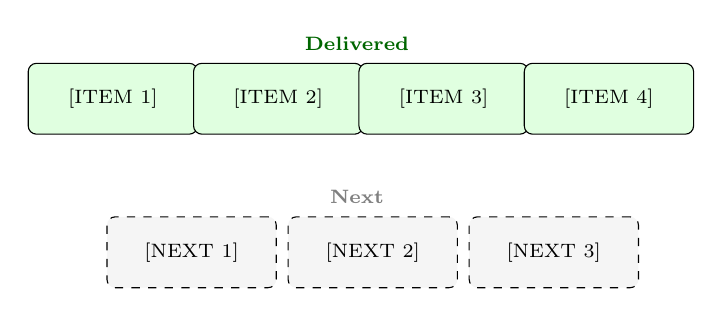
\begin{tikzpicture}[x=1cm,y=1cm]
    \node[font=\bfseries\scriptsize,green!40!black] at (3.8,2.4) {Delivered};
    \foreach \x/\label in {0.7/{[ITEM 1]},2.8/{[ITEM 2]},4.9/{[ITEM 3]},7.0/{[ITEM 4]}}
      \node[component,fill=green!12] at (\x,1.7) {\label};
    \node[font=\bfseries\scriptsize,gray] at (3.8,.45) {Next};
    \foreach \x/\label in {1.7/{[NEXT 1]},4.0/{[NEXT 2]},6.3/{[NEXT 3]}}
      \node[component,dashed,fill=gray!8] at (\x,-.25) {\label};
  \end{tikzpicture}
\end{frame}

% MODULE: conclusion -- always include
\begin{frame}{Conclusion}
  \slidepurpose{Close on the core value and evidence}{Closure}
  \begin{alertblock}{Key Takeaway}
    [ONE PRECISE SENTENCE CONNECTING PROBLEM, SOLUTION AND VALUE.]
  \end{alertblock}
  \vspace{0.3cm}
  \small
  \begin{itemize}
    \item \texttt{[CORE CONTRIBUTION]}
    \item \texttt{[VERIFIED RESULT OR LEARNING]}
    \item \texttt{[REALISTIC NEXT STEP]}
  \end{itemize}
  \centering
  \vfill
  \Large Thank you --- Questions?
\end{frame}

\end{document}
